\section{Evaluation}

Three methods of evaluation were requested for this assignment. These were:

\begin{enumerate}
	\item Produce an image of the book after each dataset is merged to produce 21 incrementally denser views of the book
	\item Compute the determinant of the covariance matrix for the corner of the cabinet closest to the viewer in each translated image to assess how closely registered the point sets are
	\item Compute the angle between the surface normal of all of the upward facing planes from the 21 images and that of the foundation image and report the mean and standard deviation of the angles
\end{enumerate}

The matlab code to perform the evaluation is shown in section \ref{EvaluationCode} of this report. The results are described in the following sections.

\subsection{Images of the book after each dataset is merged}

We produced images of the book after each dataset was merged. These images are shown in figures \ref{fig:mergedBooks1} and \ref{fig:mergedBooks2}.

\begin{figure}
	\centering
	
	\begin{subfigure}[b]{0.3\textwidth}
		\centering
		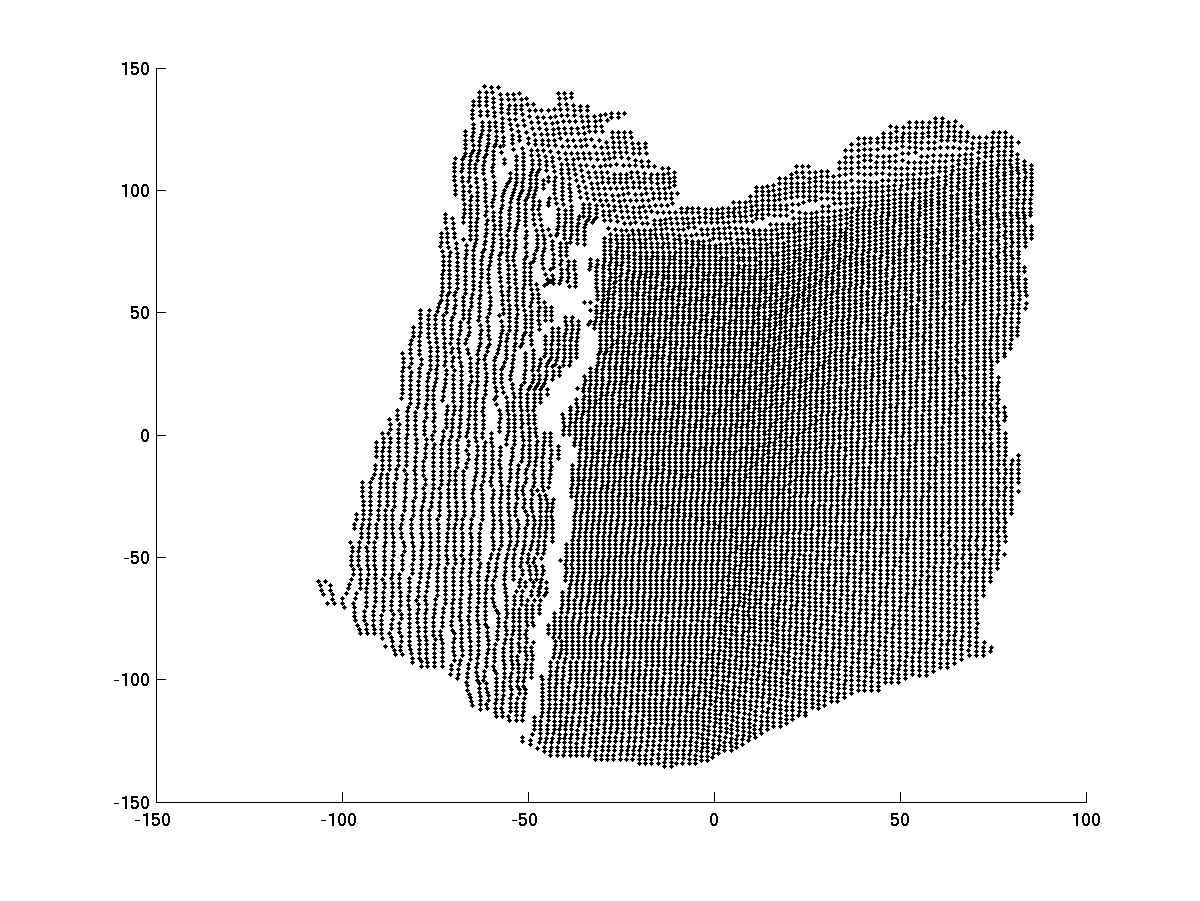
\includegraphics[width=\textwidth]{Images/Book1.png}
		\caption{}
	\end{subfigure}%
	%\hspace{1cm}
	\begin{subfigure}[b]{0.3\textwidth}
		\centering
		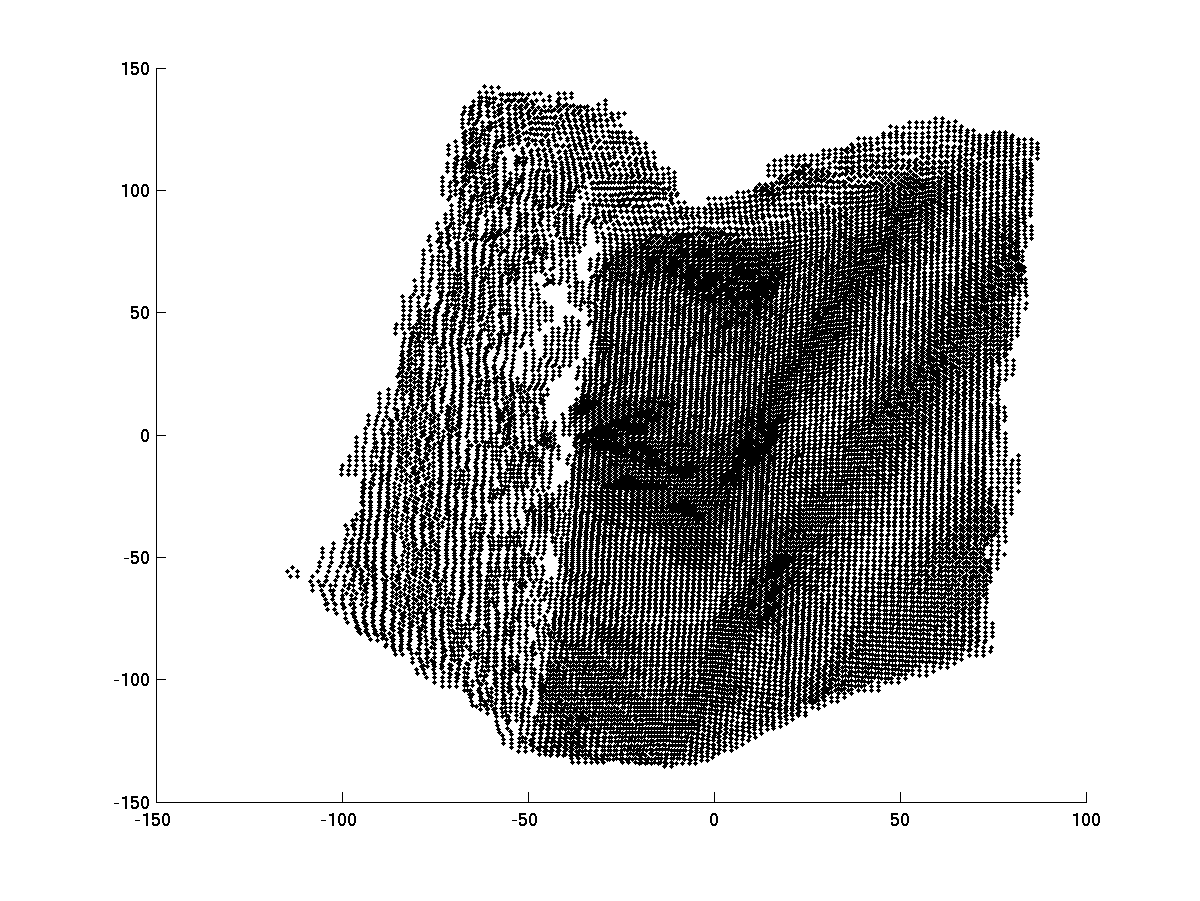
\includegraphics[width=\textwidth]{Images/Book2.png}
		\caption{}
	\end{subfigure}
	%\hspace{1cm}
	\begin{subfigure}[b]{0.3\textwidth}
		\centering
		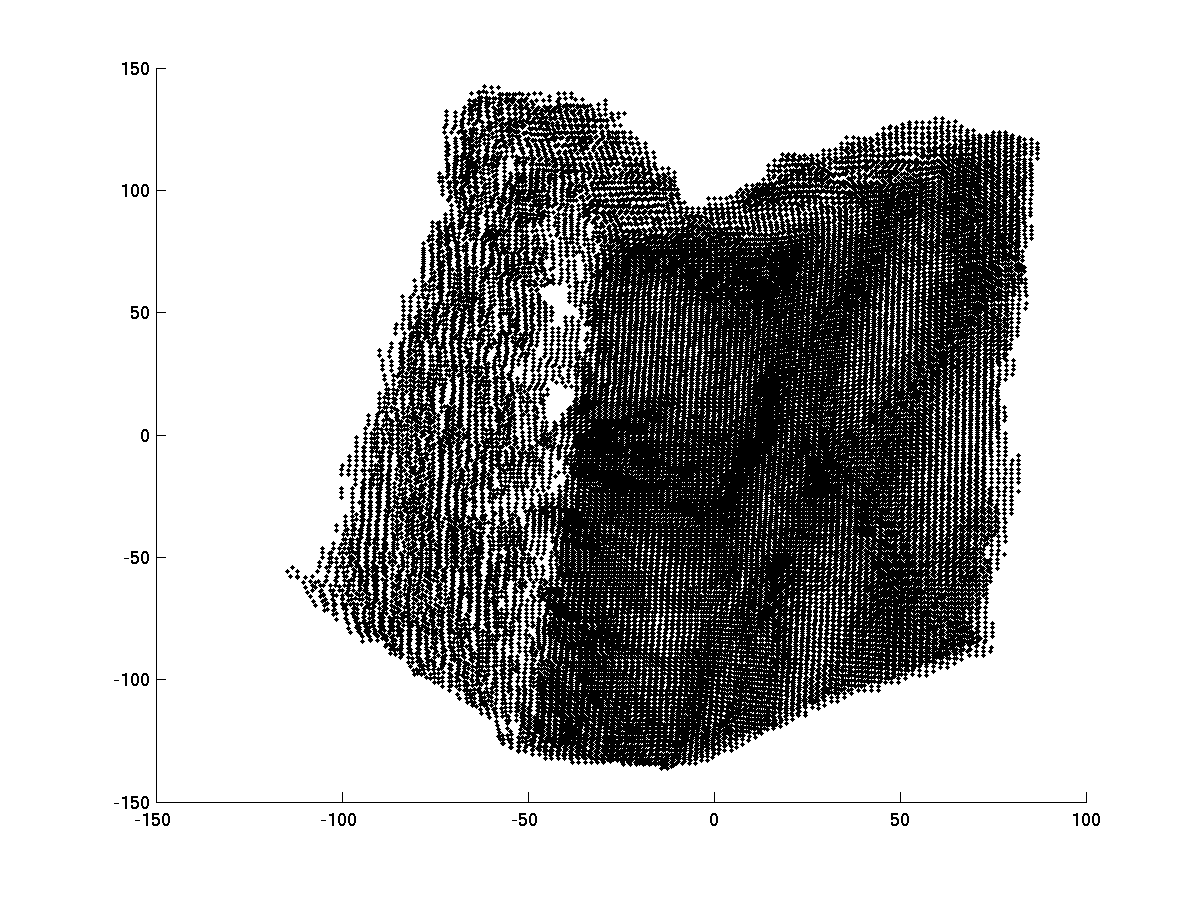
\includegraphics[width=\textwidth]{Images/Book3.png}
		\caption{}
	\end{subfigure}
	
	\begin{subfigure}[b]{0.3\textwidth}
		\centering
		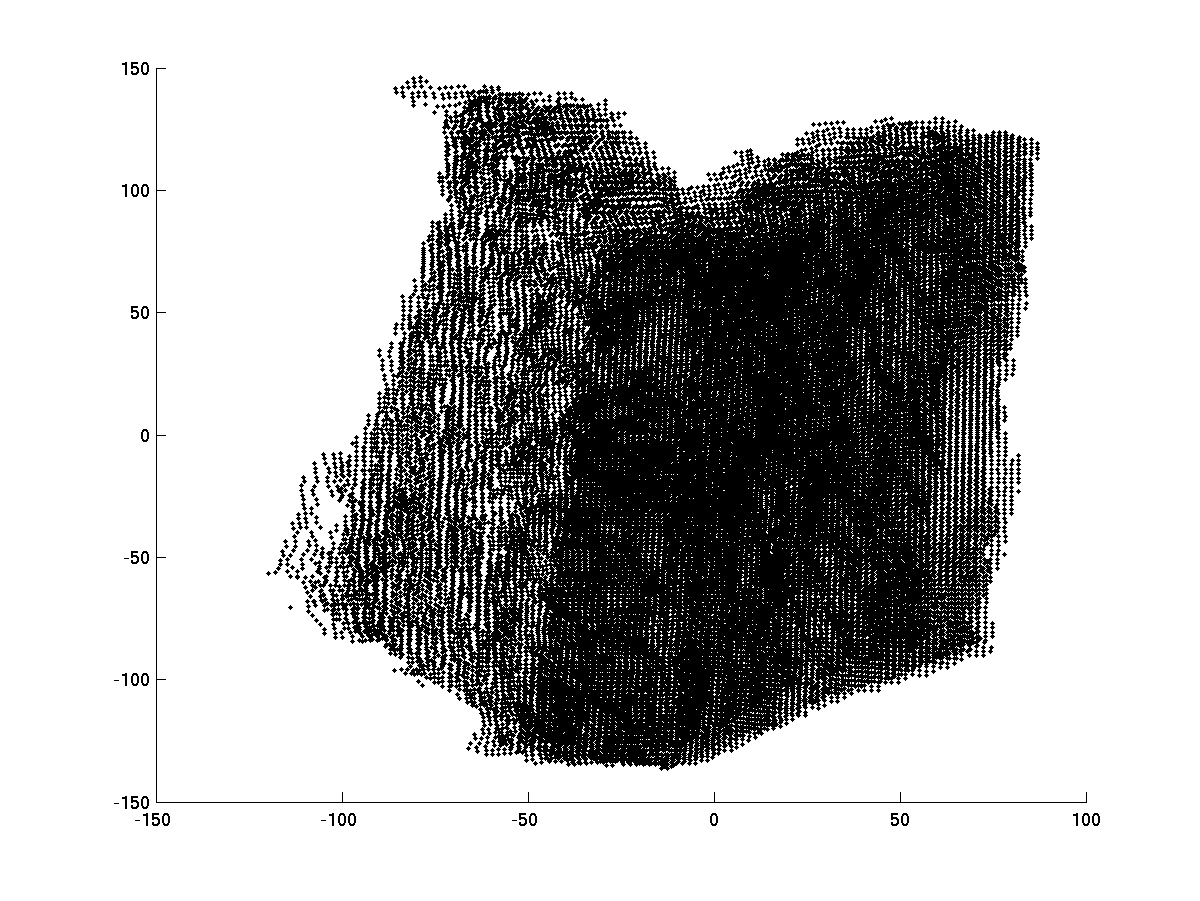
\includegraphics[width=\textwidth]{Images/Book4.png}
		\caption{}
	\end{subfigure}%
	%\hspace{1cm}
	\begin{subfigure}[b]{0.3\textwidth}
		\centering
		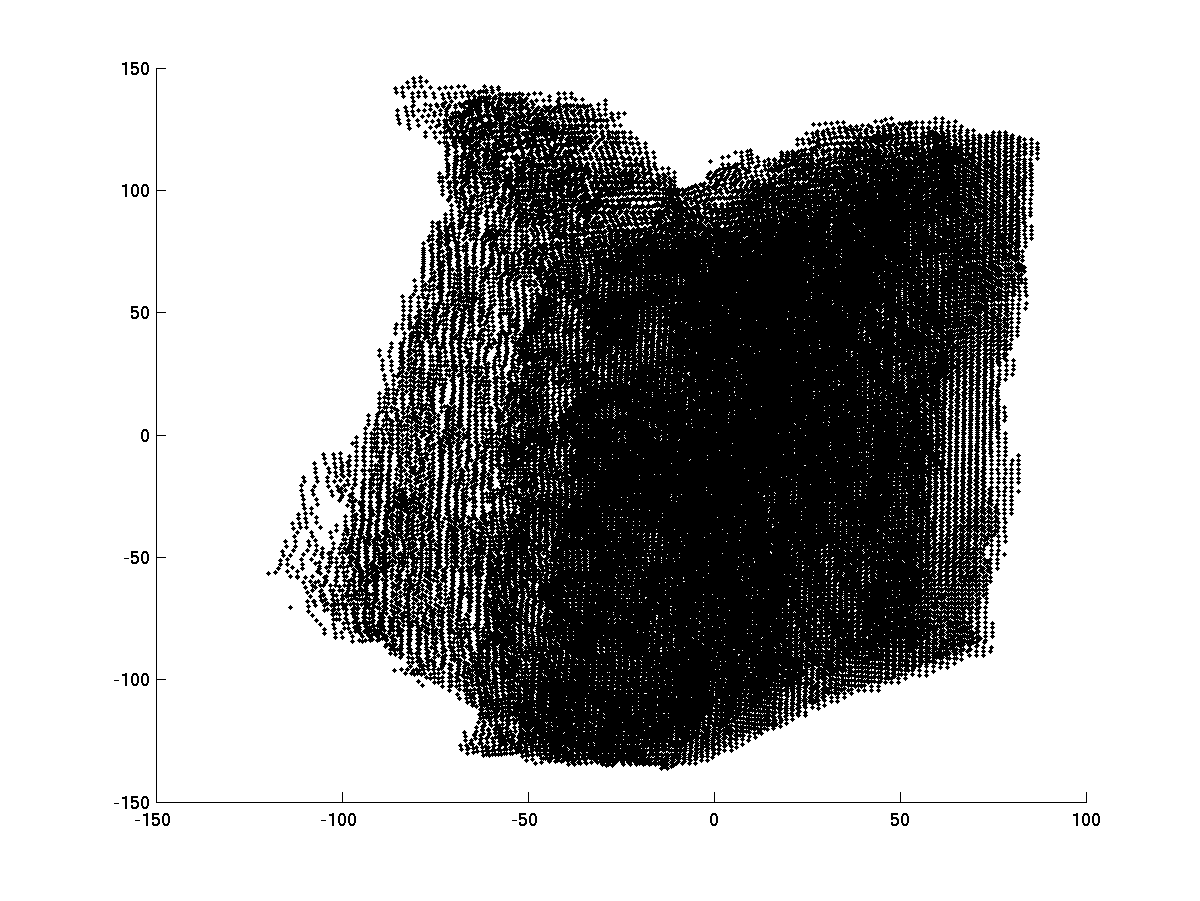
\includegraphics[width=\textwidth]{Images/Book5.png}
		\caption{}
	\end{subfigure}
	%\hspace{1cm}
	\begin{subfigure}[b]{0.3\textwidth}
		\centering
		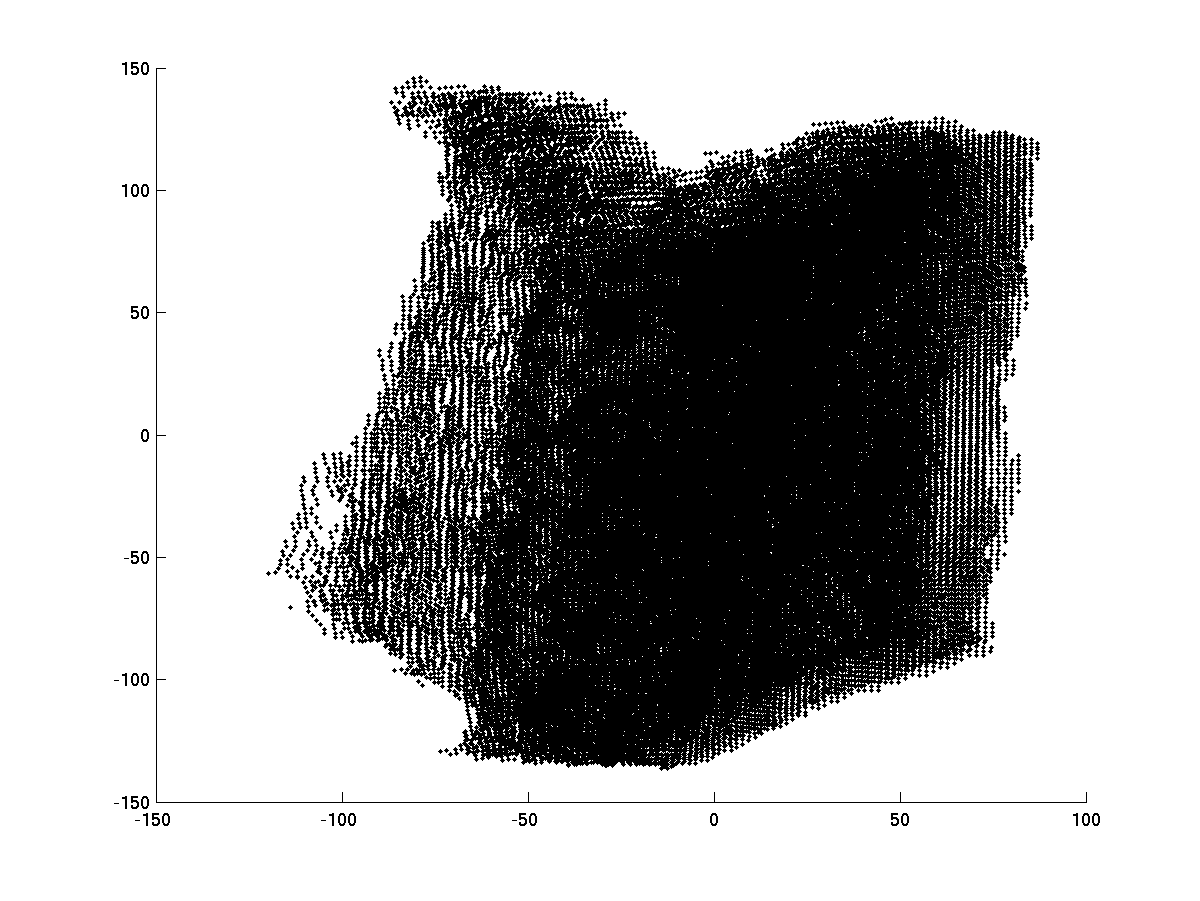
\includegraphics[width=\textwidth]{Images/Book6.png}
		\caption{}
	\end{subfigure}
	
	\begin{subfigure}[b]{0.3\textwidth}
		\centering
		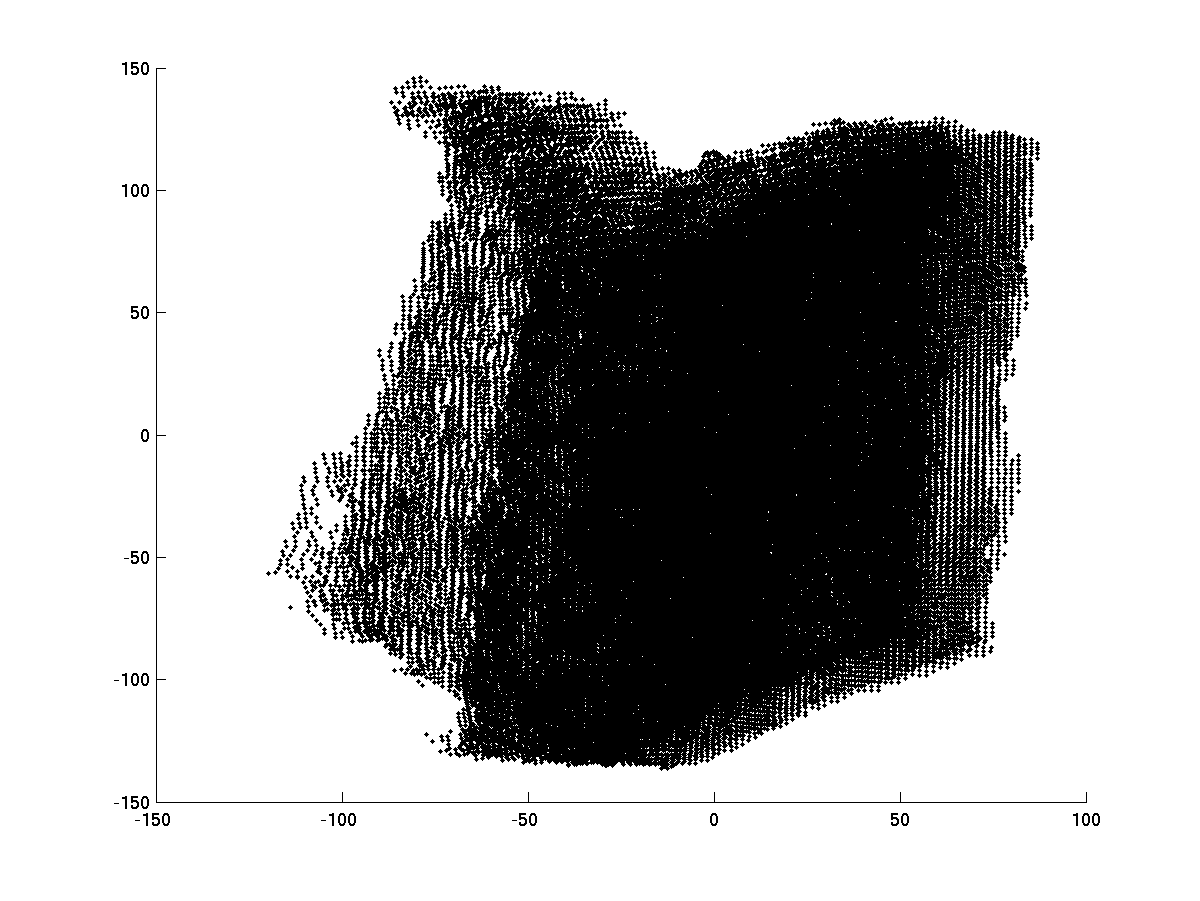
\includegraphics[width=\textwidth]{Images/Book7.png}
		\caption{}
	\end{subfigure}%
	%\hspace{1cm}
	\begin{subfigure}[b]{0.3\textwidth}
		\centering
		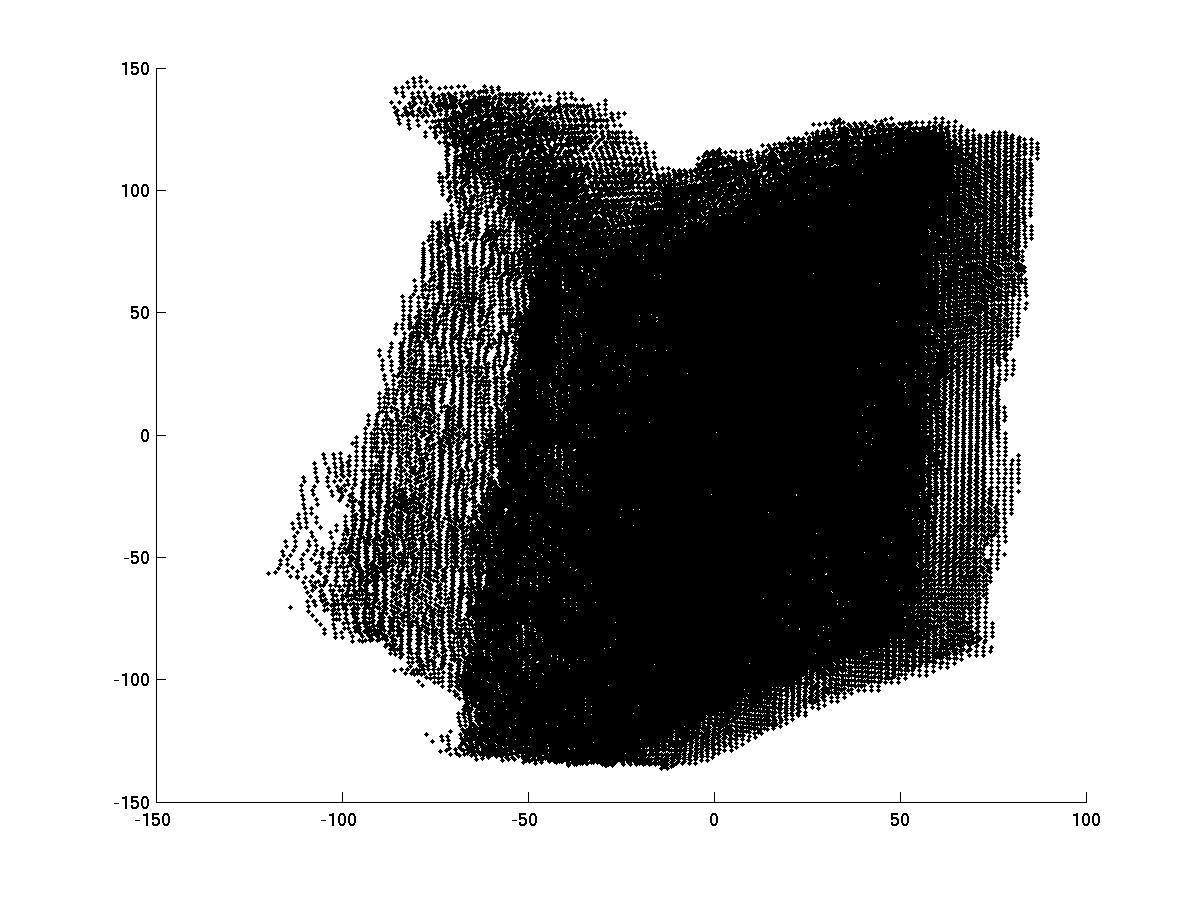
\includegraphics[width=\textwidth]{Images/Book8.png}
		\caption{}
	\end{subfigure}
	%\hspace{1cm}
	\begin{subfigure}[b]{0.3\textwidth}
		\centering
		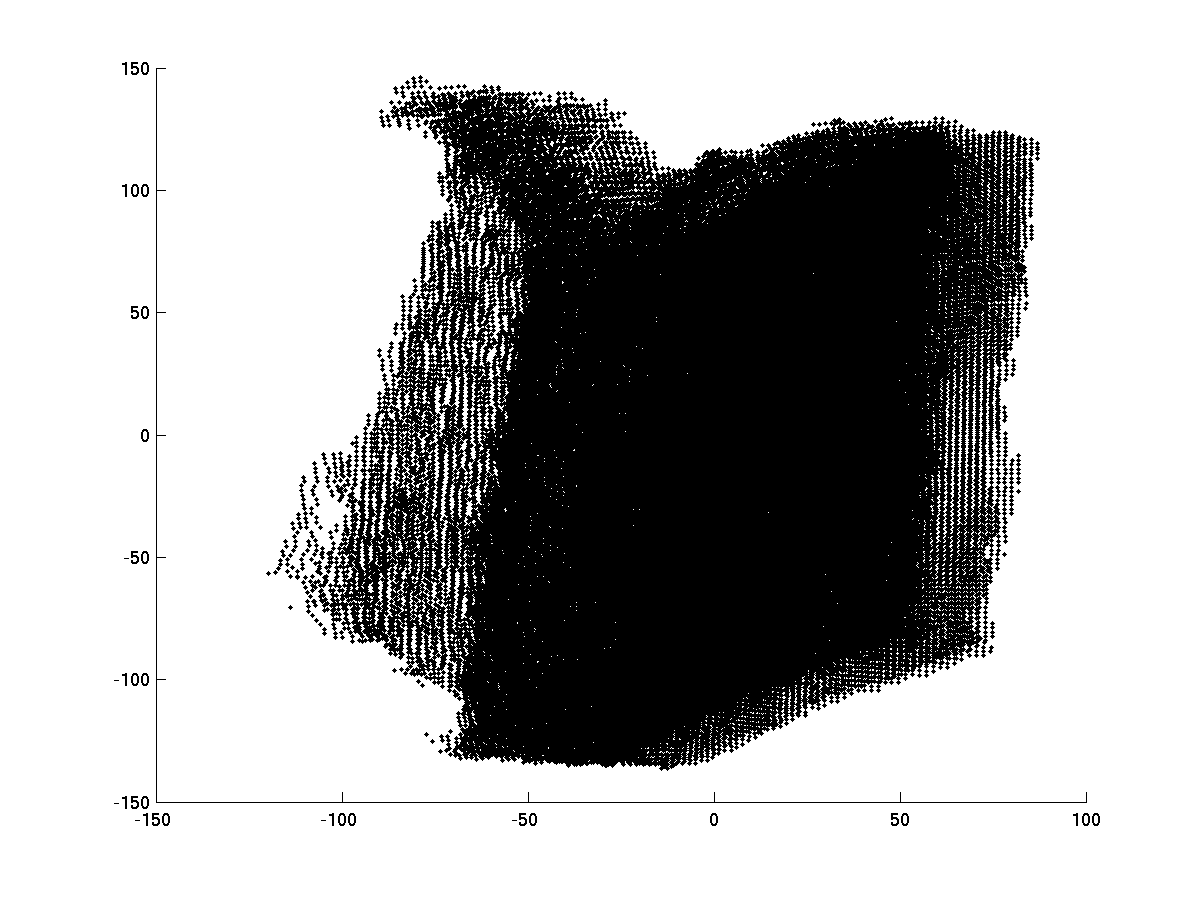
\includegraphics[width=\textwidth]{Images/Book9.png}
		\caption{}
	\end{subfigure}	
	
	\begin{subfigure}[b]{0.3\textwidth}
		\centering
		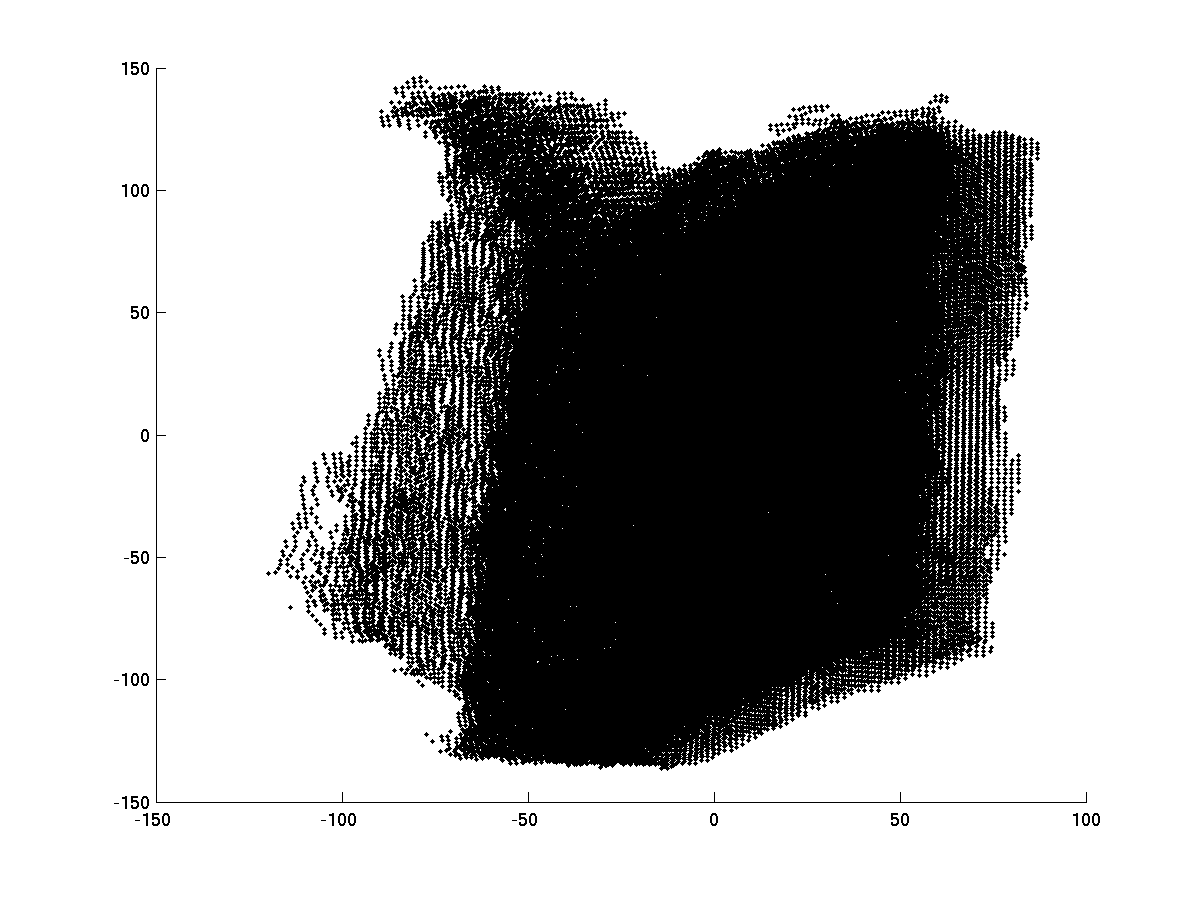
\includegraphics[width=\textwidth]{Images/Book10.png}
		\caption{}
	\end{subfigure}%
	%\hspace{1cm}
	\begin{subfigure}[b]{0.3\textwidth}
		\centering
		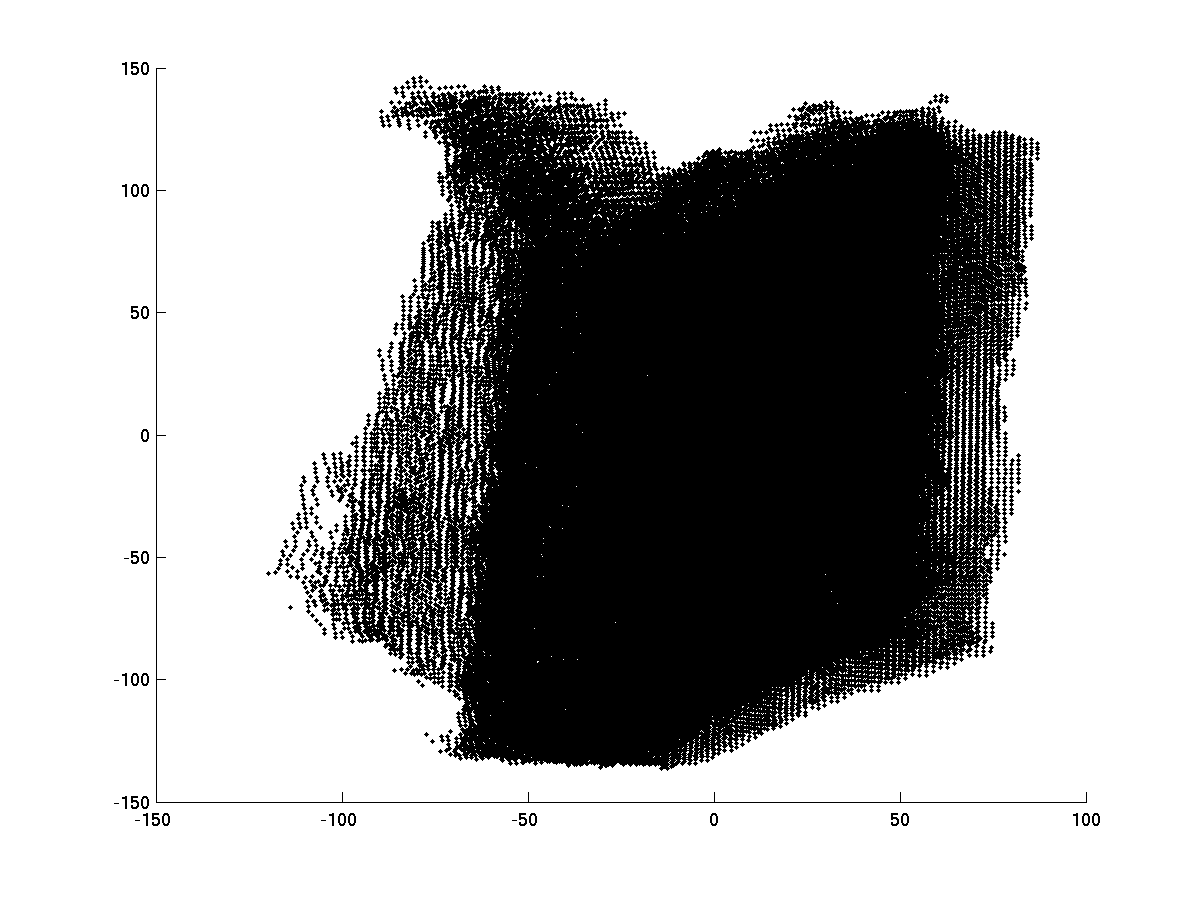
\includegraphics[width=\textwidth]{Images/Book11.png}
		\caption{}
	\end{subfigure}
	%\hspace{1cm}
	\begin{subfigure}[b]{0.3\textwidth}
		\centering
		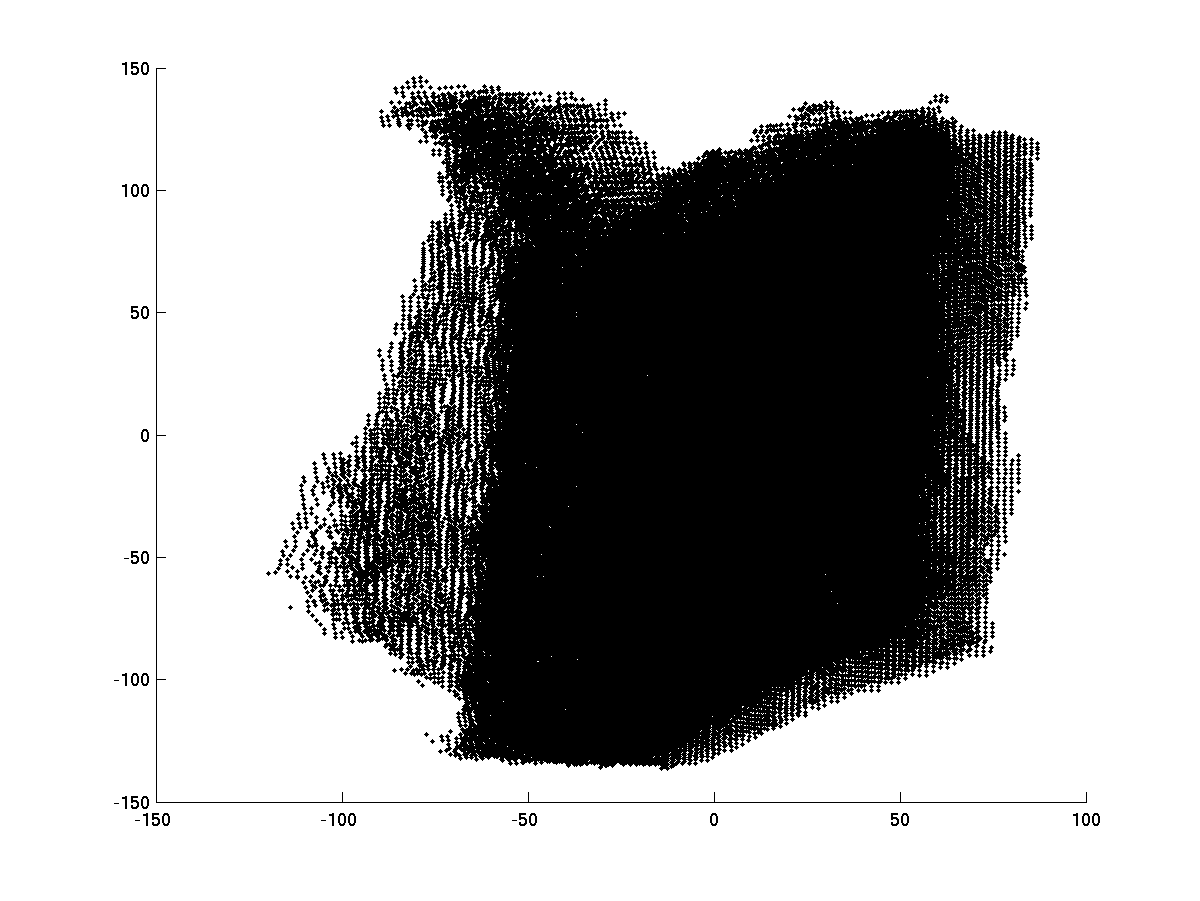
\includegraphics[width=\textwidth]{Images/Book12.png}
		\caption{}
	\end{subfigure}	
	
	\begin{subfigure}[b]{0.3\textwidth}
		\centering
		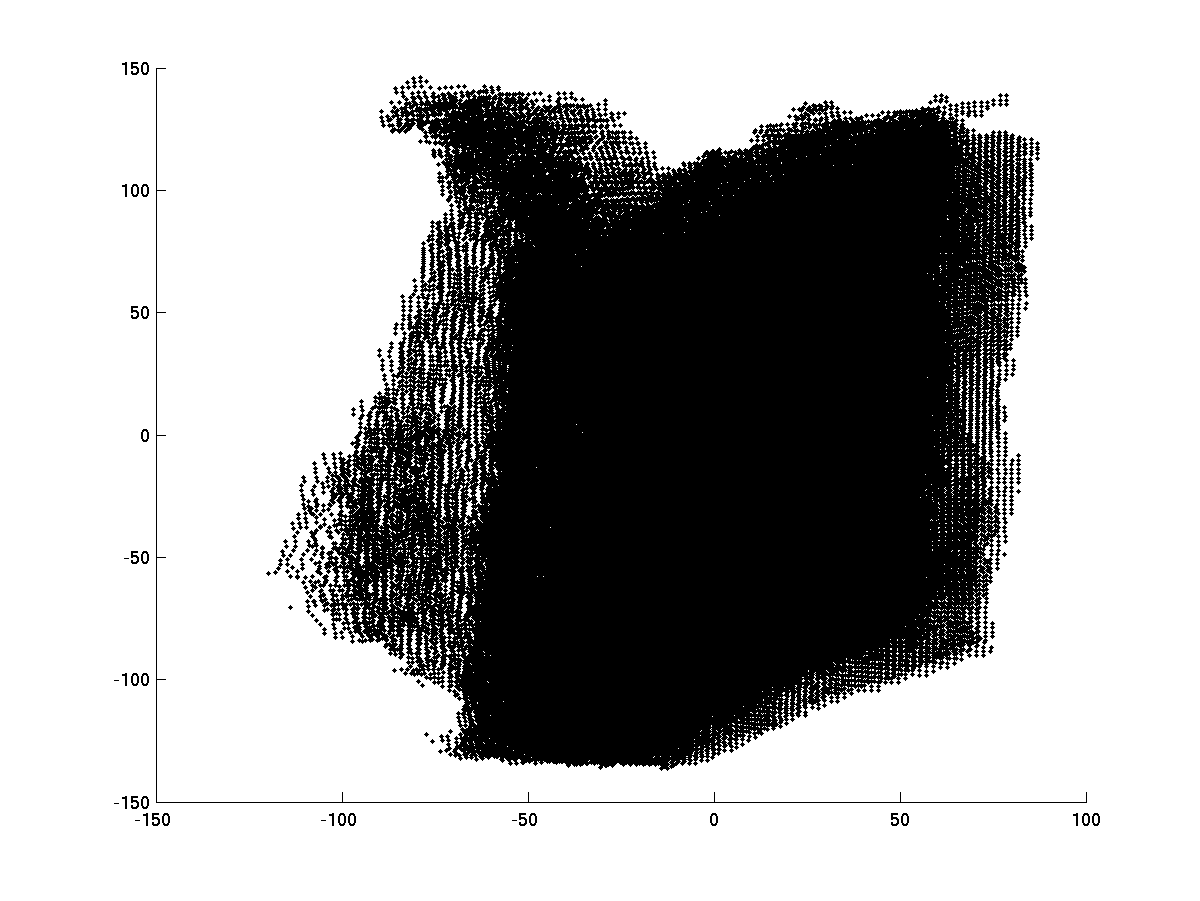
\includegraphics[width=\textwidth]{Images/Book13.png}
		\caption{}
	\end{subfigure}%
	%\hspace{1cm}
	\begin{subfigure}[b]{0.3\textwidth}
		\centering
		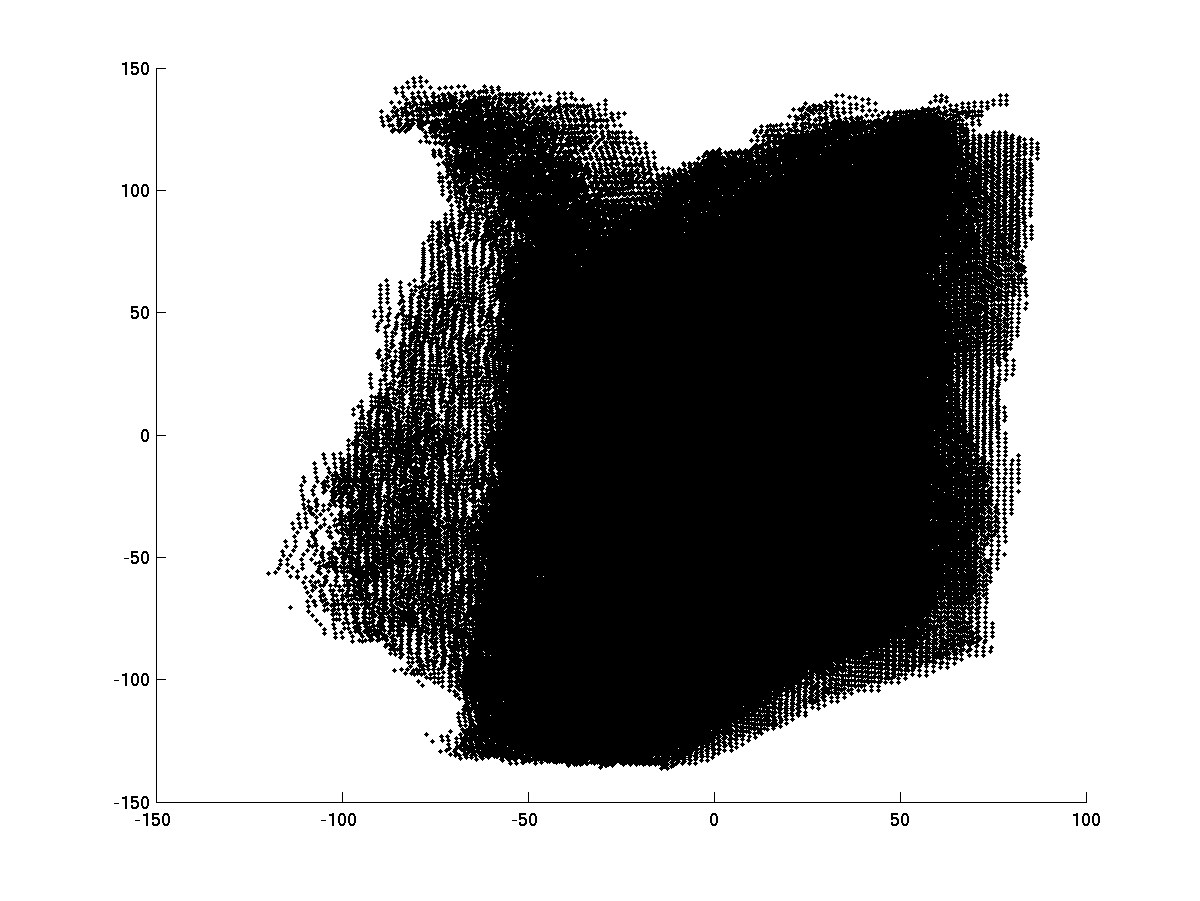
\includegraphics[width=\textwidth]{Images/Book14.png}
		\caption{}
	\end{subfigure}
	%\hspace{1cm}
	\begin{subfigure}[b]{0.3\textwidth}
		\centering
		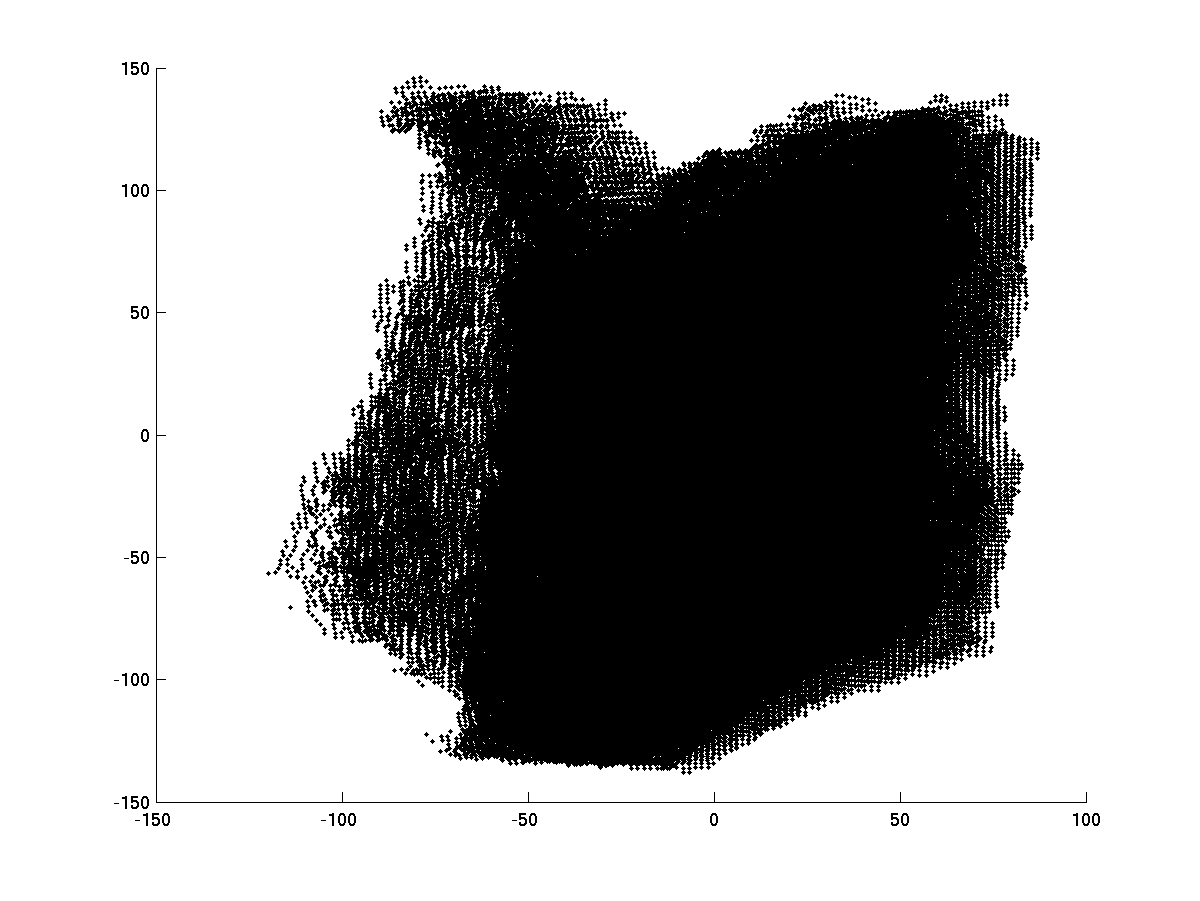
\includegraphics[width=\textwidth]{Images/Book15.png}
		\caption{}
	\end{subfigure}	
	
	\caption{Images of the book points progressively merging the first 15 frames. Image (a) is just frame 1, image (b) is frames 1 and 2, and so on. Image (o) is the result of merging images 1 to 15.}
	\label{fig:mergedBooks1}
\end{figure}

\begin{figure}
	\centering
	
	\begin{subfigure}[b]{0.3\textwidth}
		\centering
		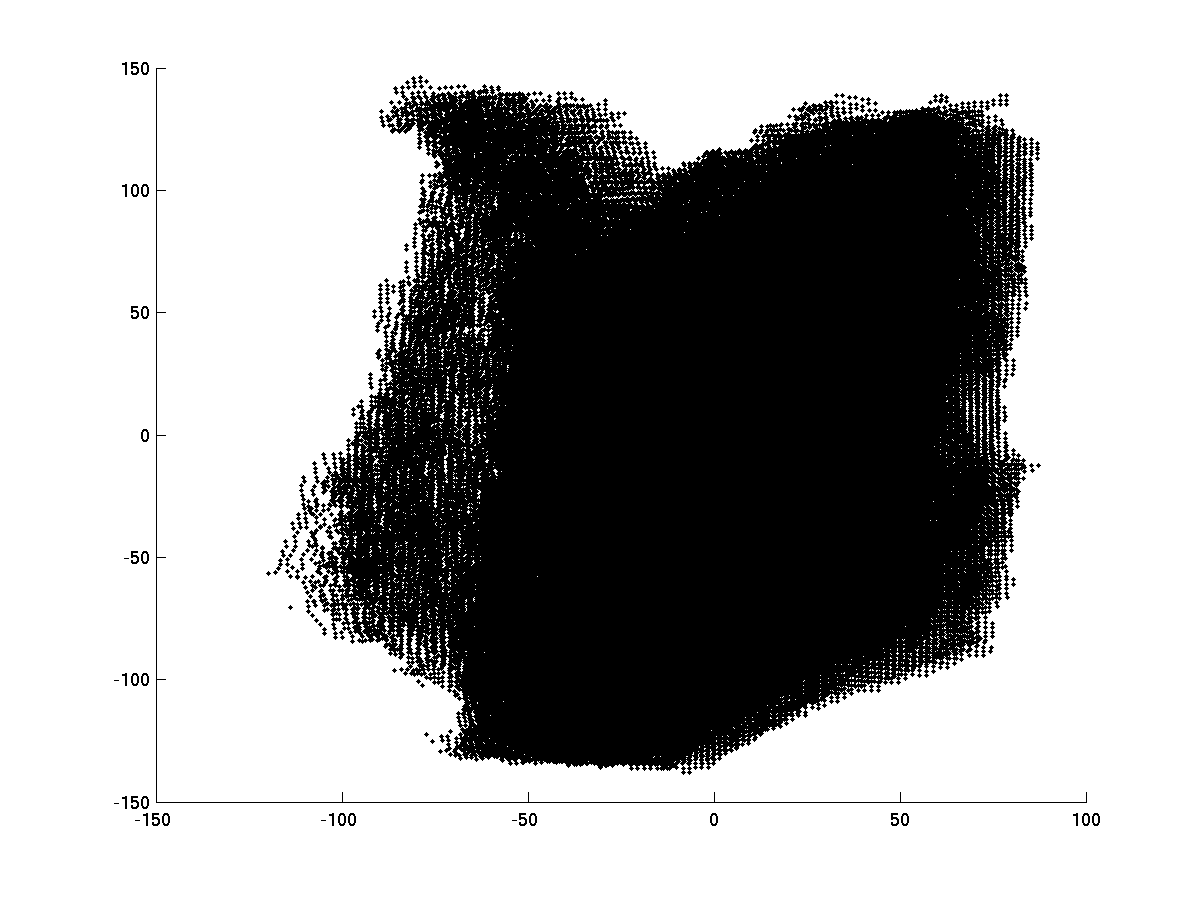
\includegraphics[width=\textwidth]{Images/Book16.png}
		\caption{}
	\end{subfigure}%
	%\hspace{1cm}
	\begin{subfigure}[b]{0.3\textwidth}
		\centering
		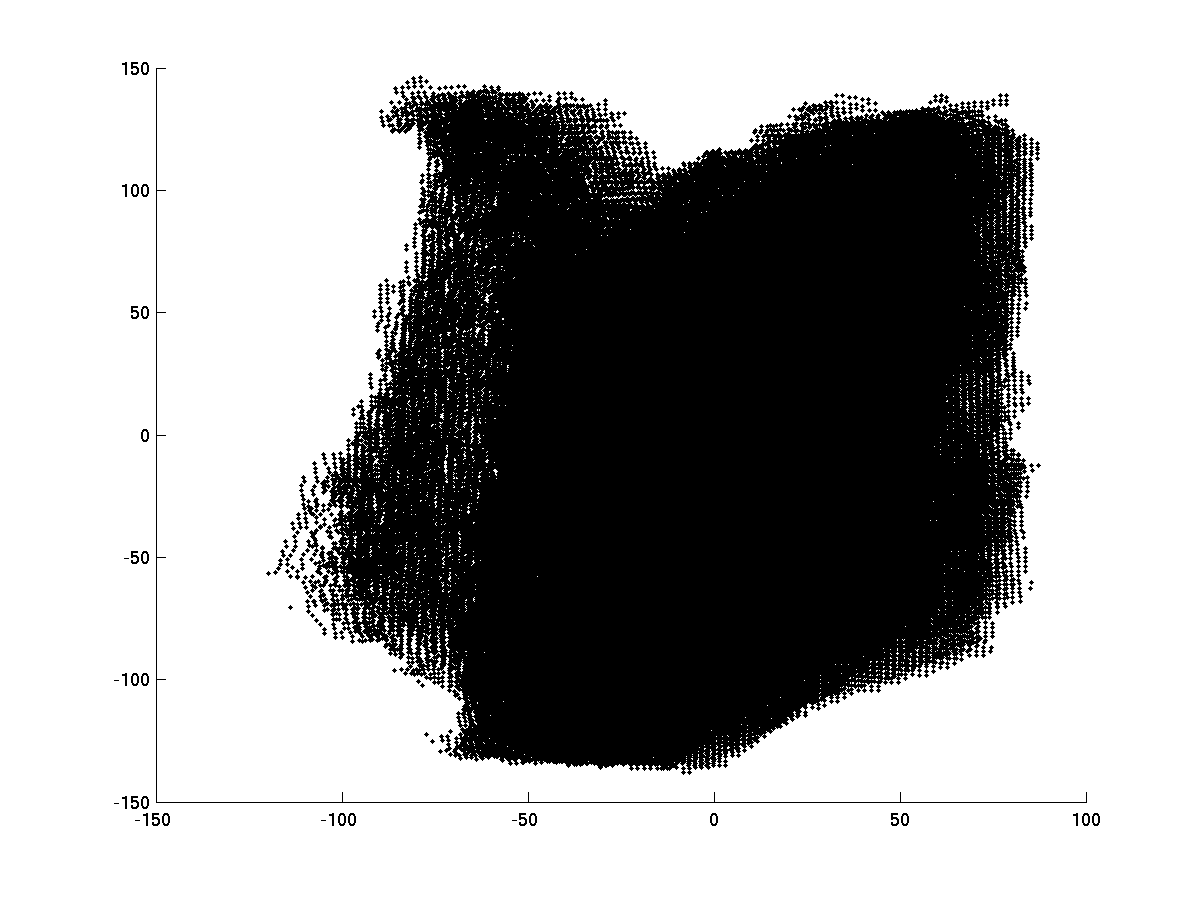
\includegraphics[width=\textwidth]{Images/Book17.png}
		\caption{}
	\end{subfigure}
	%\hspace{1cm}
	\begin{subfigure}[b]{0.3\textwidth}
		\centering
		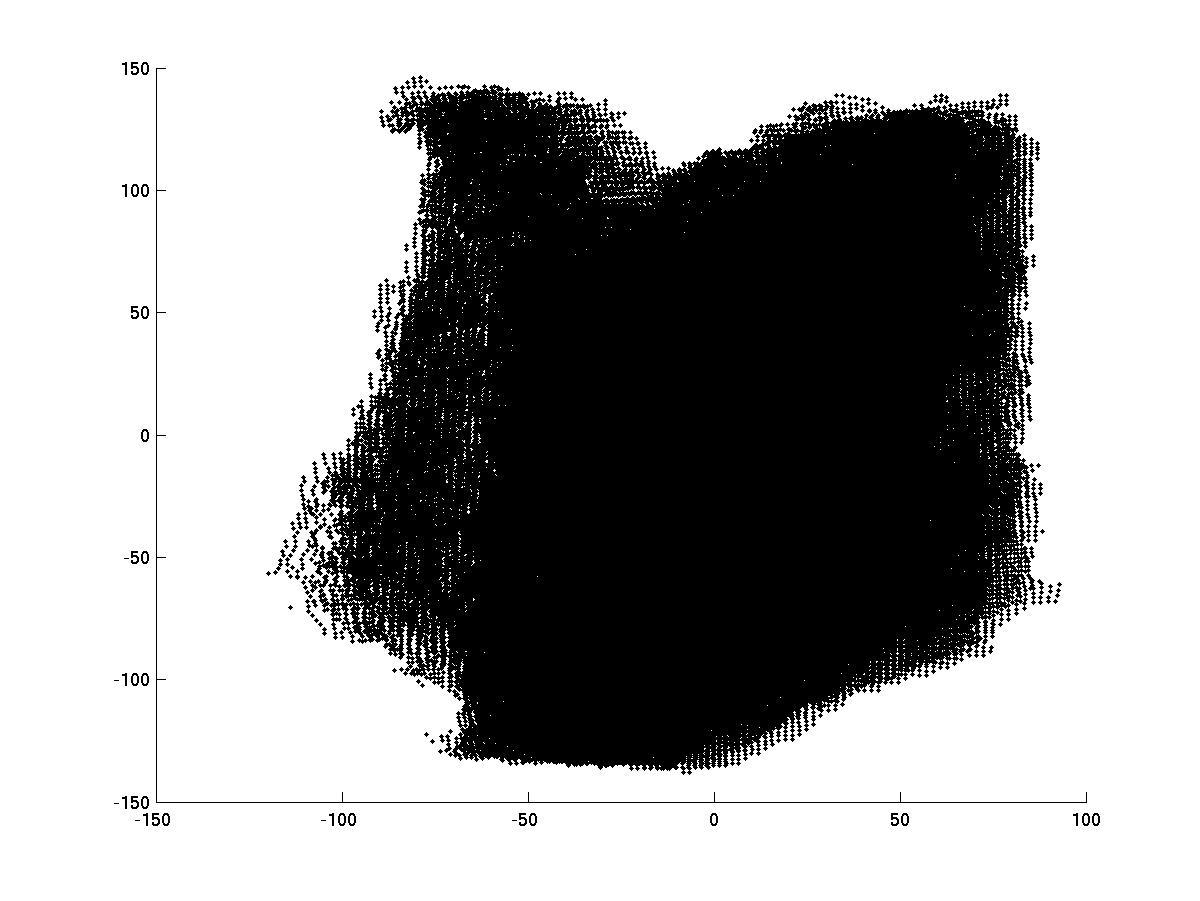
\includegraphics[width=\textwidth]{Images/Book18.png}
		\caption{}
	\end{subfigure}	
	
	\begin{subfigure}[b]{0.3\textwidth}
		\centering
		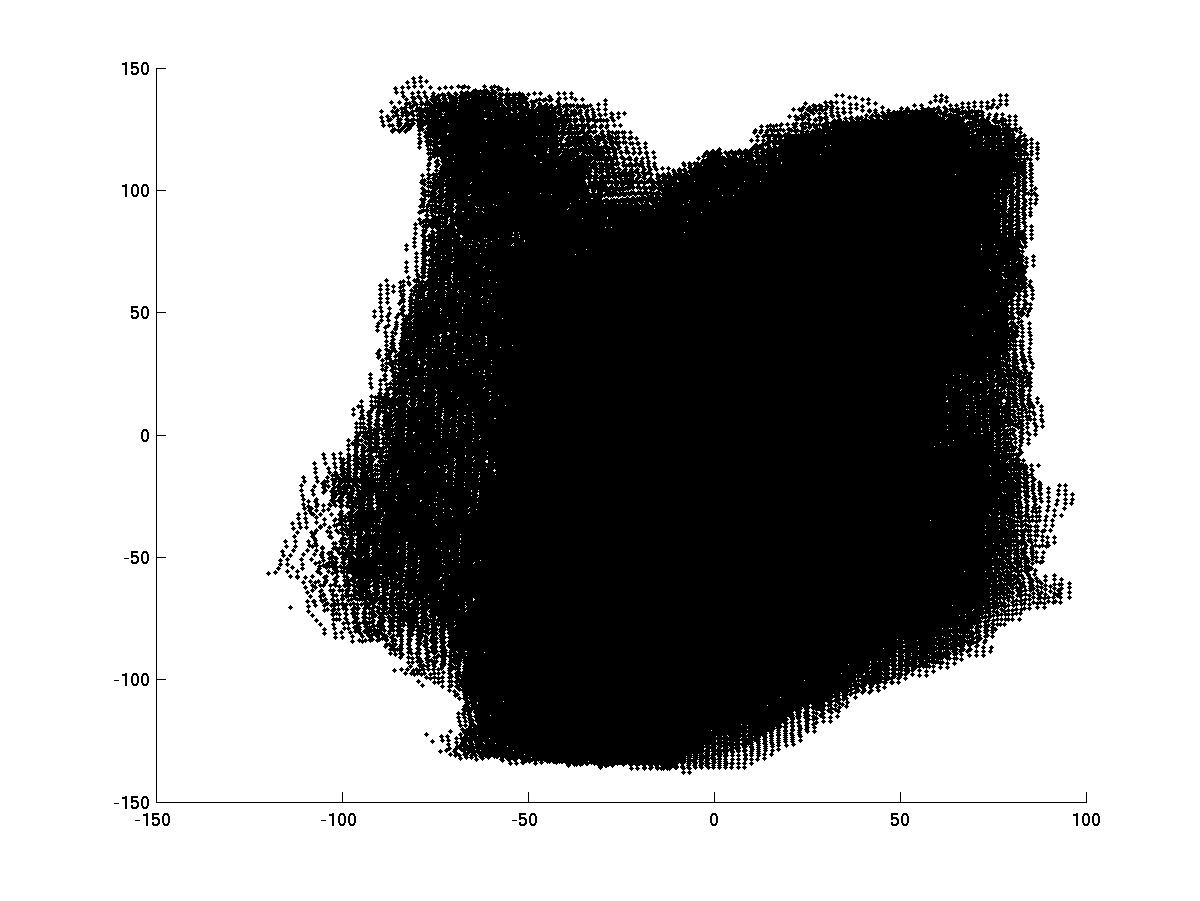
\includegraphics[width=\textwidth]{Images/Book19.png}
		\caption{}
	\end{subfigure}%
	%\hspace{1cm}
	\begin{subfigure}[b]{0.3\textwidth}
		\centering
		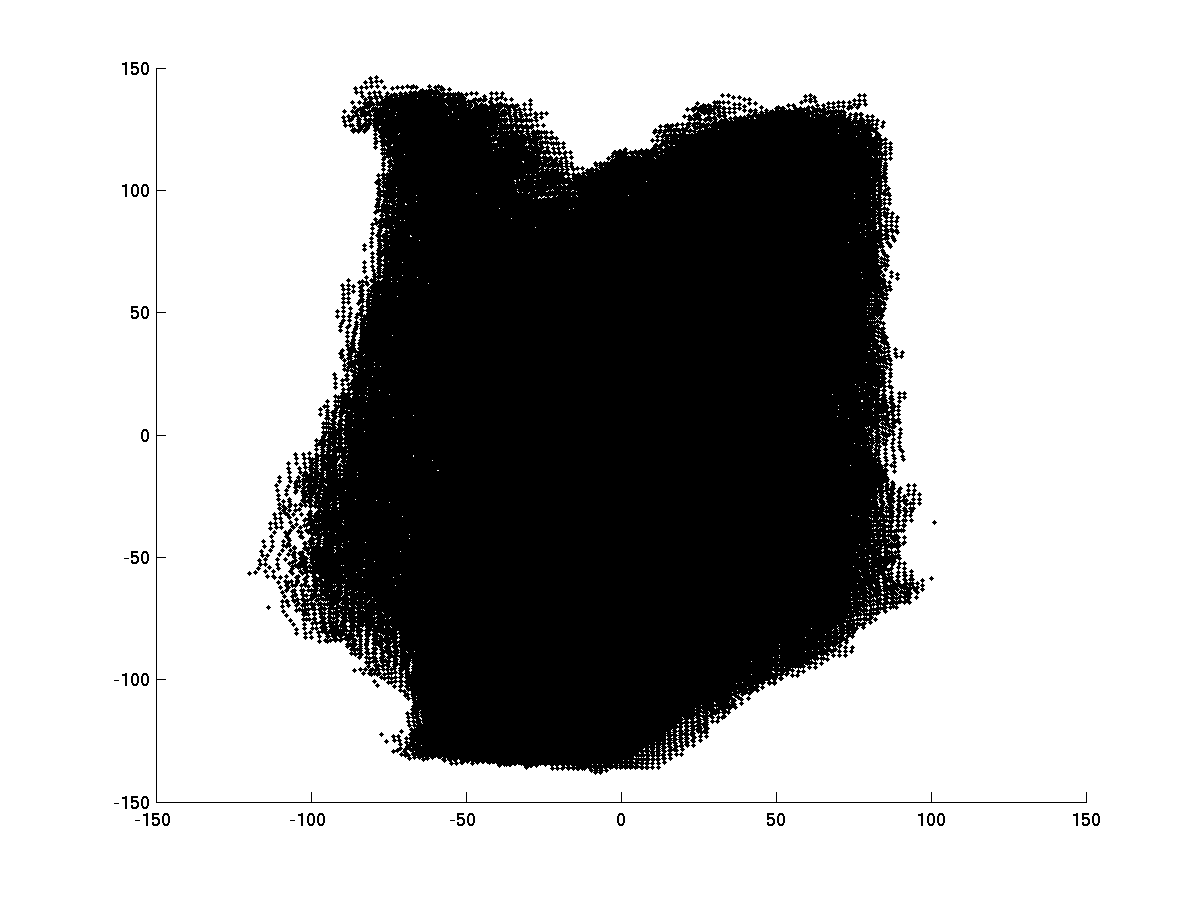
\includegraphics[width=\textwidth]{Images/Book20.png}
		\caption{}
	\end{subfigure}
	%\hspace{1cm}
	\begin{subfigure}[b]{0.3\textwidth}
		\centering
		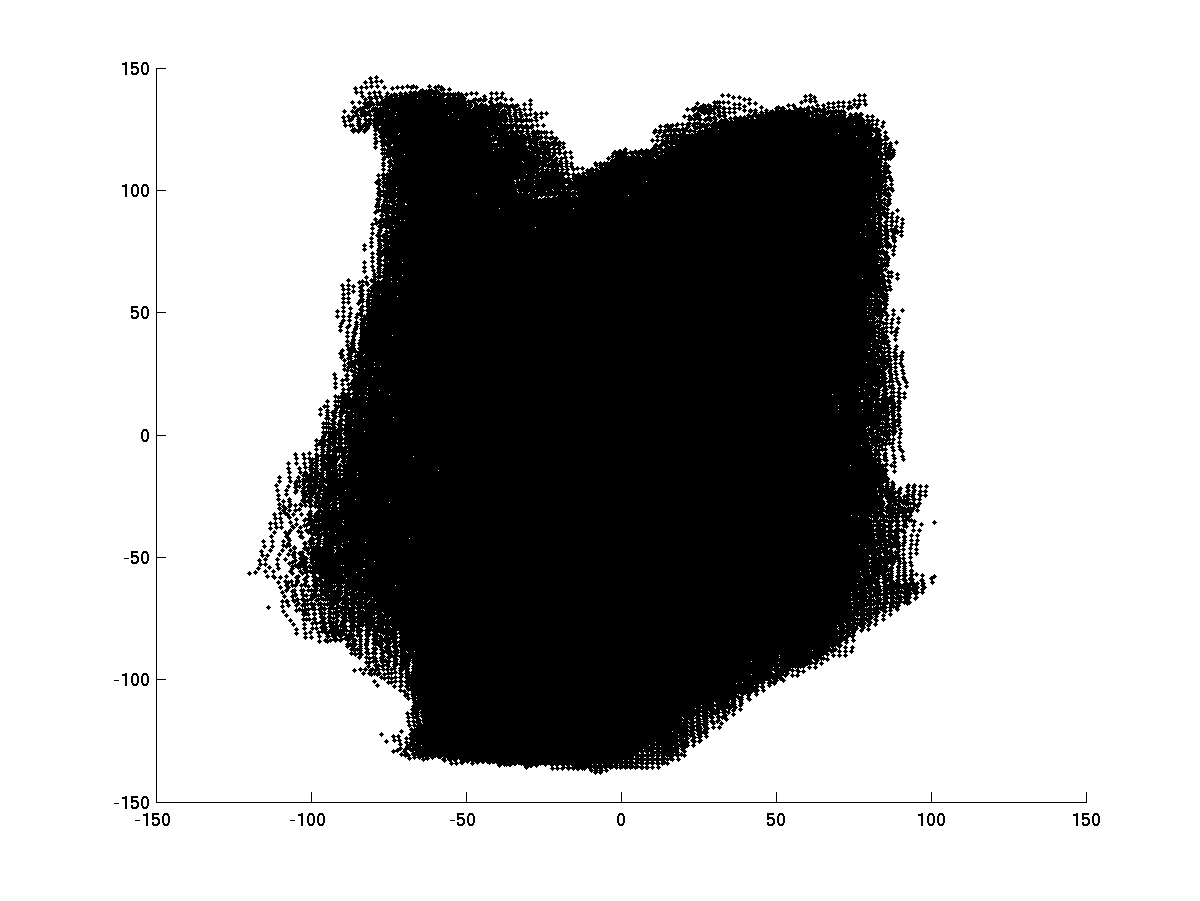
\includegraphics[width=\textwidth]{Images/Book21.png}
		\caption{}
	\end{subfigure}	
		
	\caption{Continuation of the images of the book points progressively merging the last 6 frames to the existing point cloud. Image (a) is the result of merging frames 1 to 16, image (b) is frames 1 to 17, and so on. Image (f) is the result of merging all 21 images.}
	\label{fig:mergedBooks2}
\end{figure}



\subsection{The determinant of the covariance matrix for the position of the corner of the cabinet closest to the viewer}

We computed the covariance matrix and took its determinant. The value for the determinant was $5.9359e-202$.

\subsection{The mean and standard deviation of the angles between the surface normals of all of the upward facing planes}

We computed the angles between the surface normals of the upwards facing plane of our foundation frame and the others. The average angle between the vectors was $0.0756$ and the standard deviation was $0.0599$.